\documentclass[journal]{IEEEtran}
\usepackage[T1]{fontenc}
\usepackage{amsmath,amsfonts}
\usepackage{array}
\usepackage{booktabs}
\usepackage{ragged2e}
\usepackage{tabularx}
\usepackage{url}
\usepackage{graphicx}
\usepackage{cite}
\usepackage{newtxtext,newtxmath}
\usepackage{multirow}
\usepackage[caption=false,font=footnotesize]{subfig}
\hyphenation{net-works semi-conduc-tor inter-connect chip-let photo-nic}

\newcolumntype{Y}{>{\RaggedRight\arraybackslash}X}

\begin{document}

\title{Network-on-Chip (NoC) Architectures in AI Chip and System}

\author{Man To Tam, Siu Ho Tam, Shi Long Yang, Cheuk Shing Sun, and Evan Hong Tik Lo}

\markboth{ELEC4350 Group 5 Final Project}{Tam \MakeLowercase{\textit{et al.}}: Network-on-Chip Architectures in AI Chip and System}

\maketitle

\begin{abstract}
Network-on-Chip (NoC) design has become a central concern in modern AI hardware because communication increasingly limits the scaling of neural processing systems. As AI accelerators evolve from single-die designs to heterogeneous packages with chiplets, high-bandwidth memory, and emerging optical links, the interconnect is no longer a secondary implementation detail; it is a system-level fabric that shapes latency, bandwidth efficiency, energy per bit, security, and scalability. This report surveys five directions emphasized in our group study: NoC fundamentals, AI-specific NoC optimizations, heterogeneous integration and chiplets, NoC security and trustworthiness, and emerging photonic NoC technologies. We show that AI workloads motivate multicast-aware routing and in-network compression, chiplet systems introduce a hierarchical NoC--NoP boundary that makes die-to-die communication a first-order bottleneck, and security must now be co-designed with workload structure rather than treated as an afterthought. We also compare these directions through a cross-cutting lens of scalability, programmability, and design trade-offs, and discuss why hybrid electro-photonic interconnects are promising for future global communication in large AI chips while still facing thermal and integration challenges.
\end{abstract}

\begin{IEEEkeywords}
AI accelerator, chiplet, heterogeneous integration, network-on-chip, photonic interconnect, security.
\end{IEEEkeywords}
\section{Introduction}
\IEEEPARstart{A}{I} accelerators are increasingly communication-bound. While arithmetic throughput continues to grow through parallel processing elements, tensor cores, and specialized neural processing units, overall system efficiency is often limited by how quickly weights, activations, partial sums, embeddings, and key-value cache data can move through the memory hierarchy and between compute tiles. This trend shifts the design focus from isolated compute blocks toward the communication substrate that connects them \cite{dally2001route,chen2016eyeriss}.

In this context, the Network-on-Chip (NoC) has evolved from a scalable replacement for buses and crossbars into a broader system fabric for AI chips. The same communication backbone must now support conventional on-die traffic, one-to-many data reuse in deep neural networks, inter-die movement across chiplets, trusted execution, and, in some forward-looking systems, hybrid optical links. The result is that latency, throughput, energy per bit, and trustworthiness all depend on interconnect design choices rather than on compute architecture alone \cite{bjerregaard2006survey,weerasena2024security}.

This evolution is driven by real industrial trends. Over the past five years, AI accelerator design has shifted decisively toward heterogeneity and modularity. Recent commercial accelerators from NVIDIA, AMD, Intel, and Tesla increasingly adopt multi-die or chiplet organizations connected through advanced packaging and high-bandwidth die-to-die links. At the same time, the emergence of large language models has pushed model sizes beyond what a single reticle-sized die can accommodate, making chiplet-based scaling a practical necessity rather than a design option. On a longer horizon, silicon photonics is being explored as a way to break the energy-per-bit barrier of electrical links for global on-package communication. These developments mean that the NoC is no longer just a chip-level detail; it is a system-level architectural decision that cuts across compute, memory, packaging, security, and software.

This report follows the structure emphasized in our group presentation while also following the project guidance to focus primarily on trends from roughly the past three to five years and to extract design insight rather than merely classify papers. Section~\ref{sec:fundamentals} introduces NoC fundamentals. Section~\ref{sec:aiopt} discusses AI-specific optimizations such as multicast-aware routing and compression. Section~\ref{sec:chiplet} explains why heterogeneous integration and chiplets make interconnect design even more critical. Section~\ref{sec:security} analyzes NoC security and trustworthiness in heterogeneous AI systems. Section~\ref{sec:photonic} surveys emerging photonic NoC directions. Section~\ref{sec:crosscut} then compares these directions under a unified architectural lens. We conclude by arguing that NoC design should be treated as a first-class architectural problem for scalable AI computing.

\section{NoC Fundamentals}
\label{sec:fundamentals}

\subsection{Architectural Role}

A NoC is a packet-based on-chip communication architecture that connects processing elements, SRAM blocks, accelerators, and other IP blocks through routers and links instead of relying on a shared bus. This organization improves scalability because traffic can be localized, routed hop by hop, and sustained in parallel across multiple paths. Compared with shared-bus designs, point-to-point communication and distributed arbitration reduce the collapse in local performance that often appears as system size grows \cite{dally2001route,bjerregaard2006survey}. In other words, the NoC is attractive not simply because it connects many components, but because it keeps local communication efficient even when the system becomes large and highly parallel.

\subsection{Components and Data Movement}

The basic building blocks of a NoC are resources, network interfaces, routers, buffers, and links. Resources such as processing elements or memory blocks do not communicate directly with one another; they inject and receive traffic through routers that exchange packets across the network. Router microarchitecture therefore matters: buffering policy, crossbar design, virtual channels, and speculative pipelines all affect latency and throughput \cite{peh2001delay}. In AI chips, where thousands of data transfers may be in flight simultaneously, router efficiency strongly influences the practical utilization of compute arrays.

The group presentation emphasizes a useful separation between \emph{resources} and \emph{switches}. Resources include processing elements, SRAMs, and IP cores that perform computation or store data. Switches, by contrast, provide the platform for packet exchange and play the role of routers inside the NoC. This distinction is important for AI systems because compute optimizations and communication optimizations often happen at different places: data reuse may be created by the accelerator mapping, while congestion or serialization may still emerge inside the network itself.

\subsection{Topology and Control Policies}

NoCs are attractive because they provide flexibility in topology and control policy. Common topologies include mesh, torus, binary-tree, and other hierarchical organizations, while routing may be deterministic, adaptive, centrally coordinated, or distributed. Flow control can be circuit-switched or packet-switched, depending on whether the design prefers predictable reservation or statistical multiplexing. The presentation also highlights this protocol-level freedom as a key reason NoCs can be tailored to power, performance, and area requirements rather than treated as a fixed backbone.

For AI hardware, this flexibility is valuable because dataflow patterns vary across convolution, matrix multiplication, attention, and collective communication. However, each extra hop, queue, and arbitration point also adds latency, so NoCs must balance scalability with tight timing and energy constraints \cite{chen2016eyeriss,chen2019eyerissv2}. Thus, even the ``fundamentals'' of NoC design are already shaped by AI-specific performance targets.

\subsection{Performance Metrics and Design Trade-offs}

NoC performance is characterized by several interacting metrics: zero-load latency (the delay through an otherwise idle network), saturation throughput (the injection rate at which queuing delays grow unbounded), energy per bit (including both link and router dynamic and static energy), and area overhead. For AI accelerators, two additional metrics are particularly important. The first is \emph{multicast efficiency}, which measures how effectively the network can deliver a single source value to multiple destinations without redundant transmissions. The second is \emph{communication-to-computation ratio}, which captures the balance between data movement and arithmetic throughput for a given workload mapping.

These metrics expose fundamental trade-offs. A topology with higher radix (more router ports) can reduce hop count and latency but increases router complexity and area. Virtual channels improve throughput by reducing head-of-line blocking but add buffer and scheduling overhead. Adaptive routing can avoid congestion hot-spots but may introduce out-of-order delivery that complicates the memory consistency model. For AI chips, where workloads are more predictable than in general-purpose systems, designers often choose simpler, more deterministic organizations and invest complexity instead in workload-specific optimizations such as multicast support and sparsity-aware compression. This engineering judgment---favoring workload efficiency over general-case flexibility---sets the tone for the AI-specific optimizations discussed next.

\section{AI-Specific Optimizations}
\label{sec:aiopt}

\subsection{Why General-Purpose NoCs Are Not Enough}

Traditional NoCs were largely designed around general-purpose traffic, but AI workloads have communication patterns that are both more regular and more demanding. Neural networks exhibit heavy one-to-many reuse, irregular sparsity in weights and activations, and heterogeneous precision ranging from FP16 to low-bit integer formats. If a NoC ignores these characteristics, it wastes bandwidth on redundant unicast transfers, sends zero values unnecessarily, and uses fixed-width flits even when data precision has been reduced \cite{chen2019eyerissv2,zhang2016cambriconx}.

The group presentation summarizes this mismatch clearly: general-purpose NoCs assume relatively uniform traffic, while AI workloads create repeated broadcasts, dynamic sparsity, and precision-dependent bandwidth demand. As a result, the NoC is not merely transporting tensors; it is directly participating in the efficiency of dataflow execution.

\subsection{Multicast-Aware Routing}

One key optimization direction is multicast-aware routing. In weight-stationary and input-stationary mappings, one value may need to reach many processing elements. Path-based multicast encodes multiple destinations in the packet header and forks traffic only at branching routers, making it flexible for irregular destinations at the cost of growing header overhead. In the presentation, this approach is described as a natural fit for XY-style routing with destination information carried explicitly in the packet. Tree-based multicast, by contrast, builds a spanning tree ahead of time and carries only a compact tree identifier in each packet. This lowers per-packet overhead and fits static dataflows well, but it is less adaptive when sparsity or routing demand changes at runtime. Both approaches reduce redundant traffic compared with repeated unicasts and are therefore well matched to the broadcast-heavy nature of AI accelerators.

\begin{figure*}[!t]
\centering
\subfloat[Path-based multicast: destinations are encoded in the packet header and forking occurs only at branching routers.\label{fig:pathmulticast}]{%
\begin{minipage}[c][0.25\textheight][c]{0.46\textwidth}
\centering
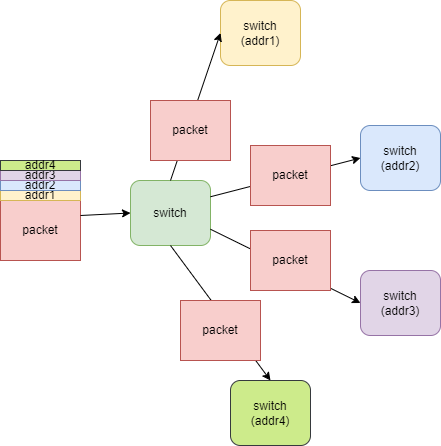
\includegraphics[height=0.23\textheight]{image/fig_path_multicast.png}
\end{minipage}}
\hfill
\subfloat[Tree-based multicast: a preconfigured spanning tree carries only a compact tree identifier in each packet.\label{fig:treemulticast}]{%
\begin{minipage}[c][0.25\textheight][c]{0.46\textwidth}
\centering
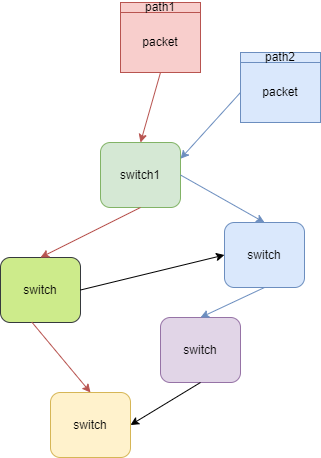
\includegraphics[height=0.23\textheight]{image/fig_tree_multicast.png}
\end{minipage}}
\caption{Comparison of two multicast strategies for AI accelerator NoCs. Path-based multicast (left) provides flexibility for irregular destination sets at the cost of header overhead, while tree-based multicast (right) minimizes per-packet metadata but requires static tree setup.}
\label{fig:multicast}
\end{figure*}

Recent trends further show that multicast support is no longer a binary choice between pure unicast and one fixed tree. Hybrid schemes can mix unicast and multicast phases, while reconfigurable fabrics and sparsity-aware pruning try to preserve the efficiency of multicast without paying the full cost under dynamic workloads. This reinforces the broader theme that AI communication increasingly rewards structure-aware networking rather than generic best-effort packet delivery.

\subsection{In-Network Compression and Sparsity Awareness}

A second major direction is in-network data compression. Sparsity-aware schemes transmit only non-zero values and their coordinates, while precision-aware schemes adapt payload width to the layer's quantization level. Model-aware techniques extend the same intuition to transformer and embedding-heavy systems by reducing communication for low-value or highly reusable data before traffic enters the network. Across these approaches, the common goal is to reduce link bandwidth demand and buffer energy without changing the algorithmic function of the model \cite{zhang2016cambriconx,jouppi2023tpuv4}. The presentation frames this as a direct response to redundancy in AI models: zeros, low-bit values, and repeated data structures all imply that raw tensor traffic is often much larger than the information that truly matters.

In practice, the challenge is that the NoC becomes more workload-aware and therefore more specialized: the better it exploits structure, the harder it may be to retain flexibility across CNNs, transformers, and future model families. AI-specific optimization therefore improves efficiency at the cost of additional router logic, metadata handling, and workload dependence.

\begin{table}[!t]
\caption{AI-Oriented NoC Optimization Directions}
\label{tab:aiopt}
\centering
\footnotesize
\setlength{\tabcolsep}{3pt}
\renewcommand{\arraystretch}{1.08}
\begin{tabularx}{\columnwidth}{p{1.5cm}Y p{1.65cm}}
\toprule
Technique & Role in AI NoCs & Main Trade-Off \\
\midrule
Path multicast & Replicates packets only at branch routers and adapts to irregular one-to-many traffic. & Header grows with fan-out. \\
Tree multicast & Uses preconfigured trees with small packet metadata for stable dataflows. & Static setup; less flexible. \\
Sparse compression & Sends only non-zero values and coordinates to cut link and buffer pressure. & Metadata and decode overhead. \\
Precision compression & Matches traffic volume to low-bit precision or data importance. & Layer-dependent scheduling. \\
\bottomrule
\end{tabularx}
\end{table}

The broader lesson is that AI-specific NoC optimization is not about making routers universally smarter; it is about co-designing communication with workload structure. Once communication is recognized as part of the dataflow, NoC features such as router replication, compression, and traffic scheduling become architectural tools rather than low-level implementation details.

\section{Heterogeneous Integration and Chiplets}
\label{sec:chiplet}

\subsection{Why Heterogeneous Integration Matters}

Heterogeneous integration changes the scope of NoC design. Instead of packing all logic onto one monolithic die, modern AI systems increasingly disaggregate compute, memory, and I/O into specialized chiplets that are assembled through advanced packaging such as 2.5D interposers or 3D stacking. This approach improves yield, lowers design cost, and allows each function to use an appropriate process node. More importantly for AI systems, it makes it possible to scale memory capacity and compute area beyond the practical limits of a single reticle \cite{yin2024review,ucie2024spec}.

The group presentation makes an important conceptual point here: heterogeneous integration is not just a packaging trick. It is a design methodology that decomposes a complex system into smaller functional blocks and reconnects them through a hierarchy of networks. For AI chips, this is especially attractive because dense compute, large SRAM, HBM, and I/O do not scale equally well on the same die or process technology.

\subsection{The NoC--NoP Boundary}

The architectural consequence is a hierarchical communication boundary between fast intra-die NoCs and slower die-to-die links. Once traffic crosses that boundary, latency and bandwidth characteristics change significantly, and the package-level network---often called a Network-on-Package (NoP)---can become the dominant bottleneck. This is particularly important for AI workloads whose collective communication and partial-sum movement already place heavy pressure on the interconnect. If mapping decisions ignore die boundaries, communication cost can dominate execution time even when each individual chiplet is efficient \cite{shao2019simba,sharma2022swap}.

This boundary is what makes chiplet NoCs fundamentally different from simply scaling a single mesh. Intra-die traffic is optimized for fine-grained communication among nearby resources, whereas inter-die traffic must tolerate higher latency, tighter energy budgets, and explicit coherence or protocol adaptation. As highlighted in the presentation, AI workloads therefore need dataflow-aware placement across chiplets so that costly cross-boundary transfers are minimized rather than treated as a scheduling afterthought.

\subsection{Advanced Packaging and Standardization}

Recent technology trends aim to narrow this gap. UCIe has become the most visible standardization effort for open die-to-die interoperability, while more advanced packaging options continue to shrink bump pitch and improve bandwidth density. The transition from 2.5D micro-bump integration toward 3D copper-to-copper hybrid bonding further increases the importance of routing across the vertical dimension, making X-Y-Z style interconnect considerations relevant to future chiplet AI systems. At the architecture level, this means that NoC design must now extend beyond on-die router layout to include D2D protocols, package topology, traffic locality, and software mapping policies.

The presentation also emphasizes the broader system consequences of this trend. Cross-die coherency protocols and logic-to-logic 3D interfaces are trying to make multi-chiplet packages behave more like virtual monolithic dies from the perspective of software. Yet the physical reality remains hierarchical. This means that future AI compilers and runtime systems must become increasingly packaging-aware if they are to realize the theoretical benefits of advanced integration.

From an AI system perspective, chiplet NoCs matter because they make scalability practical. They enable large accelerator fabrics, allow memory chiplets such as HBM stacks to sit close to compute, and support modular integration of CPU, accelerator, and I/O dies. At the same time, they expose a new design tension: the system should look unified to software, but the underlying communication substrate is increasingly heterogeneous. A successful chiplet NoC therefore requires co-design across packaging, architecture, and compiler mapping rather than simply extending a 2D mesh across more silicon.

\subsection{Key Challenges and Recent Innovations}

Table~\ref{tab:chiplet} summarizes the central technical challenges in chiplet-based AI NoCs and the most notable recent responses from industry and academia. The interoperability problem has been the most visible, and the emergence of UCIe as an open die-to-die standard represents a major step toward a multi-vendor chiplet ecosystem. However, standardization alone does not solve the bandwidth and latency disparity between intra-die and inter-die links. For large multi-chiplet AI systems, inter-chiplet communication---particularly collective traffic and data movement that repeatedly crosses die boundaries---can dominate total execution cycles \cite{shao2019simba,sharma2022swap}.

Recent research has therefore focused on communication-aware design flows. Tools such as RapidChiplet enable early-stage modeling of heterogeneous multi-chiplet networks, while dataflow-aware synthesis frameworks like SWAP co-optimize placement and routing to reduce costly cross-boundary transfers. At the physical level, the transition from passive silicon interposers to active interposers with embedded NoC routers, combined with 3D hybrid bonding, is progressively shrinking the performance gap between on-die and cross-die communication. Nevertheless, deadlock freedom across independently designed chiplets remains an open problem because traditional turn-model or virtual-channel-based guarantees do not trivially compose across heterogeneous dies with different routing policies.

\begin{table}[!t]
\caption{Key Challenges and Innovations in Chiplet-Based AI NoCs}
\label{tab:chiplet}
\centering
\footnotesize
\setlength{\tabcolsep}{3pt}
\renewcommand{\arraystretch}{1.08}
\begin{tabularx}{\columnwidth}{p{1.7cm}Y p{1.5cm}}
\toprule
Challenge & AI System Impact & Recent Solutions \\
\midrule
Interoperability & Vendor IP cannot interoperate easily without common D2D interfaces. & UCIe; CXL-over-UCIe bridging. \\
Bandwidth gap & Cross-die traffic can dominate runtime in communication-heavy mappings. & Hierarchical routing, active interposers, 3D hybrid bonding. \\
Deadlock & Independent chiplets can break end-to-end routing assumptions. & Global NoP protocols, modular turn models. \\
Thermal stress & Boundary links raise package hot-spot density in 2.5D/3D systems. & Power-gated links, thermal-aware TSV placement. \\
Workload mapping & Poor placement pushes too much traffic across die boundaries. & RapidChiplet; SWAP-style mapping. \\
\bottomrule
\end{tabularx}
\end{table}

Thermal and power considerations add another layer of complexity. Driving signals across chiplet boundaries, whether through silicon interposers, organic substrates, or 3D TSVs, consumes significantly more energy per bit than on-die communication. In stacked configurations, this energy becomes concentrated heat that must be managed through power-gated links and thermal-aware physical design. Finally, testability and yield management become more difficult because a single failed D2D link can compromise an entire multi-chiplet package, making known-good-die (KGD) strategies and post-assembly repair mechanisms essential for practical deployment.

\section{NoC Security and Trustworthiness}
\label{sec:security}

\subsection{Why Security Is Now a NoC Problem}

As AI systems scale into heterogeneous and multi-chiplet platforms, the NoC becomes an attack surface as well as a transport fabric. Modern on-chip networks may carry proprietary model weights, embeddings, intermediate activations, user inputs, and memory traffic associated with secure execution. This makes confidentiality, integrity, availability, and supply-chain trust central interconnect concerns rather than purely software-level concerns \cite{charles2022survey,weerasena2024security}.

\subsection{Threats in Heterogeneous AI Systems}

AI traffic is especially exposed because it is structured and repetitive. Convolution, matrix multiplication, attention, and collective communication often produce highly predictable patterns in timing, link utilization, and buffer occupancy. That predictability makes traffic analysis and side-channel inference easier than in irregular general-purpose workloads. In heterogeneous AI systems, additional risks include congestion-based denial-of-service, malicious third-party IP blocks, and compromised chiplet routers or memory interfaces \cite{pasricha2022electronic,sarihi2021survey}. The same open standards that enable chiplet interoperability also widen the trust boundary if die authentication and secure boot mechanisms are weak.

This is one of the clearest cases where the presentation adds AI-specific nuance to the broader literature. A generic NoC may already be vulnerable to snooping, congestion, or malicious routing state changes. An AI NoC, however, exposes structured dataflows that can reveal model architecture, layer behavior, or even user-dependent inputs through side channels. The network is therefore not only a path for attacks but also a source of information leakage.

\begin{table}[!t]
\caption{Representative NoC Security Risks in AI Systems}
\label{tab:security}
\centering
\footnotesize
\setlength{\tabcolsep}{3pt}
\renewcommand{\arraystretch}{1.08}
\begin{tabularx}{\columnwidth}{p{1.7cm}Y p{1.5cm}}
\toprule
Threat & Impact in AI & Typical Defense \\
\midrule
Side-channel analysis & Can reveal model structure or input-dependent behavior from timing and congestion. & Traffic shaping, randomized routing. \\
Congestion / DoS & Can trigger latency spikes and throughput collapse in shared inference. & QoS-aware routing, anomaly monitoring. \\
Trojanized IP & Can corrupt routing state or leak traffic through third-party logic. & Authentication, secure boot, monitors. \\
Untrusted chiplets & Expands the trust boundary across standardized D2D links. & D2D attestation, chiplet root-of-trust. \\
\bottomrule
\end{tabularx}
\end{table}

\subsection{Workload-Aware Defenses}

Recent designs suggest a shift from generic protection to workload-aware protection. Trusted execution support for NPUs, as seen in architectures such as TNPU and sNPU, moves secure enclaves closer to the accelerator itself instead of relying entirely on the host CPU \cite{lee2022tnpu,feng2024snpu}. GuardNN and Securator similarly show that protecting AI data paths requires balancing encryption, integrity verification, and latency sensitivity rather than simply inserting heavyweight cryptographic blocks everywhere \cite{hua2022guardnn,shrivastava2023securator}. The key insight is that AI chips cannot afford security mechanisms that destroy TOPS/W, so interconnect protection must be co-designed with predictable dataflow and traffic locality.

The defense landscape can be organized into several complementary directions. \emph{Cryptographic protection}---including link-layer encryption, packet authentication codes, and integrity trees---provides strong confidentiality and integrity guarantees but adds latency and energy overhead that may be unacceptable on critical data paths. \emph{Access control and isolation} mechanisms partition the NoC into secure and non-secure regions at the router level, preventing unauthorized IP blocks from observing or interfering with sensitive traffic. \emph{Secure routing} techniques, such as randomized path selection and oblivious routing, reduce the predictability that side-channel attackers rely on, though they may reduce throughput. \emph{Runtime monitoring} deploys hardware sensors and machine-learning-based anomaly detectors throughout the network to identify congestion attacks, abnormal traffic patterns, or thermal side-channel activity in real time.

For heterogeneous chiplet systems, an additional layer of trust management is required. Chiplet root-of-trust mechanisms establish a hardware-anchored chain of trust from die authentication at boot time through ongoing runtime attestation. Secure interposer monitors can observe D2D traffic for protocol violations without adding latency to the data path. However, these mechanisms must themselves be lightweight and verifiable, because a compromised security monitor becomes a single point of failure for the entire package.

The presentation argues that this predictability is both a risk and an opportunity. Structured communication makes side-channel leakage easier, but it also enables lighter-weight protection mechanisms such as dataflow-aware obfuscation, selective isolation, and accelerator-local trusted execution. A further nuance is that AI workloads exhibit \emph{phase behavior}: training has different security requirements and traffic patterns than inference, and batch inference differs from interactive serving. This temporal structure opens the door to adaptive security policies that apply stronger protection only when and where it is needed, amortizing the overhead over the full execution. This trade-off is likely to define the next stage of secure AI interconnect design.

\section{Emerging Technologies: Photonic NoC}
\label{sec:photonic}

\subsection{Why Photonic NoCs Are Attractive}

Photonic NoCs are motivated by the scaling limits of electrical interconnects. As AI models grow larger and more distributed within a package, long-distance communication demands high bandwidth density and low energy per bit that conventional metal wiring struggles to deliver. Optical waveguides and wavelength-division multiplexing (WDM) offer a promising alternative by allowing multiple data streams to share the same physical channel through different wavelengths \cite{vantrease2008corona,pan2009firefly}.

The fundamental advantage is physical. In electrical links, energy per bit grows with distance because repeaters, equalization, and termination all consume power. In an optical waveguide, once light is coupled into the channel, propagation loss is far less sensitive to distance. This makes photonic links especially attractive for the global communication paths that span an entire chip or package, where electrical alternatives would require many power-hungry repeater stages. Furthermore, WDM allows a single waveguide to carry tens of wavelengths simultaneously, each modulated at tens of gigabits per second, creating aggregate bandwidth densities that electrical links cannot match within practical power budgets.

\subsection{Hybrid Electro-Photonic Organization}

For AI accelerators, photonic links are particularly attractive for global traffic. Long-distance broadcasts, reductions, and chip-scale synchronization can benefit from the lower propagation delay and higher aggregate bandwidth of optical channels. However, the most practical near-term direction is not a fully optical chip. Instead, the presentation's emphasis on hybrid electro-photonic NoCs is well justified: optical links are best suited to long-distance, high-bandwidth communication, while electrical links remain preferable for short, local transfers where simple CMOS routing is still more efficient \cite{pasricha2022electronic,weerasena2024security}.

This hybrid organization maps naturally onto the hierarchical communication patterns of AI workloads. Local communication within a compute cluster---such as partial-sum exchange between nearest-neighbor multiply-accumulate units---is dominated by short, frequent, latency-sensitive messages that are well served by electrical NoCs. Global communication---such as broadcast of filter weights to all tiles, all-reduce across the full accelerator, or chiplet-to-chiplet data movement---involves longer distances and higher aggregate bandwidth demand, making it a strong candidate for photonic paths. The key architectural question is where to place the electro-optical interfaces so that conversion overhead does not erase the benefits of optical transport.

\begin{table}[!t]
\caption{Hybrid Electro-Photonic Link Roles in AI Accelerators}
\label{tab:photonic}
\centering
\footnotesize
\setlength{\tabcolsep}{3pt}
\renewcommand{\arraystretch}{1.08}
\begin{tabularx}{\columnwidth}{p{1.55cm}Y p{1.8cm}}
\toprule
Link Type & Best Role & Example Traffic \\
\midrule
Optical links & Long-distance global traffic with high bandwidth demand. & Weight broadcast, all-reduce, chiplet-to-chiplet tensors. \\
Electrical links & Short local transfers among nearby components and routers. & Partial sums, local activations, control traffic. \\
\bottomrule
\end{tabularx}
\end{table}

\subsection{Open Challenges}

The remaining challenges are substantial. Photonic components are thermally sensitive: even small temperature variations shift resonator wavelengths and can detune WDM channels, requiring active thermal stabilization that consumes power and adds control complexity. Insertion loss accumulates at every bend, coupler, and waveguide crossing, limiting the practical number of optical hops before signal regeneration is needed. Crosstalk between adjacent wavelengths or waveguides can degrade signal integrity, especially in dense WDM systems. And perhaps most critically, integration with standard CMOS manufacturing remains expensive and complex because photonic devices require different material properties and process steps than logic transistors.

These issues mean that photonic NoCs are best viewed as an emerging complement to electrical NoCs rather than an immediate replacement. Even so, they represent an important direction because they align closely with the communication profile of future large-scale AI systems: frequent global exchange, strict energy budgets, and growing pressure on package-level bandwidth. Recent demonstrations of silicon photonic interposers and micro-ring-based WDM links in research environments suggest that the technology is maturing, but the gap between laboratory demonstration and volume manufacturing remains wide \cite{pasricha2022electronic,weerasena2024security}.

\section{Cross-Cutting Comparison and Open Challenges}
\label{sec:crosscut}

\subsection{A Unified Comparison Lens}

The five directions discussed above are often studied in different communities, but for AI chips they address the same system-level question: how can communication scale with model size, accelerator parallelism, and deployment complexity? Fundamental NoC design provides the baseline packet fabric. AI-specific optimizations reduce redundant traffic within that fabric. Chiplet integration extends the communication scope beyond a single die. Security research ensures that the same fabric remains trustworthy under sharing and heterogeneity. Photonic research explores whether the physical medium itself must change as bandwidth demand continues to rise. Seen this way, these directions are not isolated topics; they are successive layers in the evolution of AI interconnect design.

\begin{table*}[!t]
\caption{Cross-Cutting Comparison of NoC Directions for AI Chips}
\label{tab:crosscut}
\centering
\footnotesize
\setlength{\tabcolsep}{4pt}
\renewcommand{\arraystretch}{1.08}
\begin{tabularx}{\textwidth}{p{2.55cm}Y Y p{2.0cm}}
\toprule
Direction & Main Benefit & Main Cost or Limitation & Relative Maturity \\
\midrule
Core NoC fundamentals & Scalable on-chip baseline for AI communication. & Still exposed to congestion and topology mismatch at extreme scale. & Mature, still evolving \\
AI-specific multicast and compression & Cuts redundant traffic via reuse, sparsity, and mixed precision. & Adds workload-specific logic and metadata handling. & Active research; selective deployment \\
Chiplet-based NoC and NoP & Scales beyond reticle limits and enables heterogeneous integration. & Pays D2D latency, thermal, and mapping costs. & Rapid industrial adoption \\
Secure and trustworthy NoC & Protects model data and shared-service availability. & Adds energy, latency, and trust-management overhead. & Emerging, increasingly urgent \\
Hybrid electro-photonic NoC & Improves bandwidth density for long-range global traffic. & Constrained by thermal tuning, loss, and integration cost. & Experimental and emerging \\
\bottomrule
\end{tabularx}
\end{table*}

Table~\ref{tab:crosscut} highlights a useful pattern. The closer a technique is to the AI workload itself, the more efficiently it can remove unnecessary communication, but the more specialized it becomes. By contrast, more general communication substrates retain flexibility yet often pay larger energy or latency penalties. This explains why recent research increasingly combines multiple strategies at once: for example, chiplet systems with workload-aware mapping, secure accelerators with traffic-aware protection, or photonic fabrics used only for bandwidth-dominant global paths \cite{jouppi2023tpuv4,ucie2024spec,weerasena2024security}.

\subsection{Shared Open Challenges}

Several open challenges cut across all NoC directions. First, the communication bottleneck continues to grow as AI models move from CNNs toward transformers, mixture-of-experts systems, and recommendation workloads with large embeddings. These workloads create more collective communication, larger working sets, and stronger pressure on bandwidth and memory locality. Second, there is a persistent trade-off among performance, energy, security, and programmability. Mechanisms that improve one dimension often stress another, especially in edge systems with strict power budgets or in datacenter systems that must maintain high utilization.

Third, heterogeneity is becoming the norm rather than the exception. Modern AI platforms increasingly mix CPUs, NPUs, HBM stacks, chiplets, and possibly near-memory or photonic components. This means the NoC can no longer be optimized in isolation; it must be co-designed with packaging, memory systems, software scheduling, and trust boundaries. Fourth, benchmarking remains fragmented. Different papers report different workloads, traffic assumptions, precision levels, and evaluation metrics, which makes direct comparison difficult. A trend that appears dominant in one benchmark suite may look less compelling under another. Fifth, industry deployment is moving faster than academic standardization. Open die-to-die standards, large multi-chip modules, and optical attachments are already reshaping practical AI systems, while many academic models still assume simpler substrates \cite{yin2024review,weerasena2024security}.

\subsection{The Convergence Toward Hierarchical Communication}

When these challenges are considered together, a clear convergence emerges. The most promising designs for future AI chips are neither purely electrical nor purely optical, neither fully homogeneous nor arbitrarily heterogeneous, and neither maximally general nor narrowly specialized. Instead, they organize communication into a hierarchy that matches the natural structure of AI workloads. At the finest granularity, within a compute cluster, short electrical links provide low-latency, high-throughput local communication for partial sums, activations, and control messages. At the chip level, multicast-aware and sparsity-aware NoCs reduce redundant traffic among tiles executing the same layer. At the package level, standardized D2D interfaces and hierarchical NoP routing manage longer-distance traffic across chiplets with tolerable latency and energy overhead. At the global level, photonic paths are reserved for the most bandwidth-intensive collective operations. Security controls are layered correspondingly: light-weight traffic shaping within trusted clusters, stronger encryption and authentication at chip boundaries, and die attestation at the package level.

This hierarchical view explains why no single NoC technique can claim to be the solution. The design space is too multi-dimensional, and the constraints change with scale. What it also suggests is that the most impactful research contributions in the coming years will likely be those that address the \emph{interfaces} between these layers: how to decide which traffic goes to which layer, how to maintain end-to-end guarantees when each layer has different reliability and security properties, and how to expose enough information to compilers and runtimes so that data placement and communication scheduling can be optimized jointly.

These challenges suggest a broader research insight: future AI interconnects will likely be \emph{hierarchical, workload-aware, and heterogeneous by default}. In other words, the best NoC for future AI chips may not be a single uniform fabric, but a layered communication system in which local electrical NoCs, package-level chiplet links, security controls, and selected photonic paths are co-optimized around model behavior and deployment goals.

\section{Conclusion}

NoC architecture has moved to the center of AI chip design. At the foundational level, it provides the scalable packet-based communication needed to replace buses and crossbars. At the workload level, it can exploit multicast, sparsity, and mixed precision to reduce unnecessary traffic. At the system level, chiplets and heterogeneous integration transform NoC design into a package-level problem in which die boundaries, D2D standards, and compiler mapping strongly influence performance. At the trust level, the same interconnect becomes a shared attack surface that must protect sensitive model and user data. Finally, at the technology frontier, hybrid electro-photonic fabrics suggest a path beyond the bandwidth and energy limits of purely electrical links.

The common theme across these directions is that communication is no longer a background service for AI hardware. It is a first-class architectural resource whose design determines whether future AI systems can scale efficiently, securely, and economically. The strongest takeaway from our survey is therefore not that one NoC technique will dominate all future systems, but that successful AI chips will increasingly depend on communication co-design across workload, architecture, packaging, and trust.

Looking forward, several research directions appear especially promising. First, the integration of communication-aware compilation with chiplet-scale NoP design remains an open problem: compilers and runtimes need richer abstractions for die boundaries, link bandwidth, and latency so that data placement decisions can be optimized alongside routing. Second, security mechanisms must continue to evolve from static, uniform protection toward adaptive, workload-phase-aware policies that apply heavyweight protection only when and where the risk justifies the cost. Third, as photonic interconnects mature from laboratory demonstrations toward manufacturing, the architectural community needs better models for hybrid electro-photonic design-space exploration that account for thermal tuning power, insertion loss budgets, and CMOS integration cost alongside traditional NoC metrics. Finally, the trend toward open chiplet ecosystems and standardized D2D interfaces creates an opportunity for the research community to define open NoC benchmarks, traffic traces, and evaluation frameworks that can produce more consistent and comparable results across different studies.

That is the point at which NoC research stops being a narrow interconnect topic and becomes a core discipline of AI chip and system design. In a field where model sizes double every few months and deployment scenarios span from milliwatt-scale edge sensors to megawatt-scale datacenters, the communication fabric is not just infrastructure. It is the architecture.


\newpage
\bibliographystyle{IEEEtran}
\bibliography{references}

\end{document}
